\section{Einleitung}
\label{kap:ein}
% note-fp: intressante asatz, mit dere kurze ifüherig, I hät da glaub zümme gno mitem 1.1, aber I würds mol dinne loh, mol luege was dini betreuer dage
\newcommand{\br}[1]{\textbf{\textcolor{red}{#1}}}
\newcommand{\strike}[1]{\sout{#1}}
\newcommand{\st}[1]{\sout{#1}}

In diesem Kapitel wird die Auftragsgeberfirma Colomba Link vorgestellt. Es wird die Ausgangslage beschrieben und das zu lösende Problem wird eingeführt. Es werden grundlegende Begriffe definiert, die in dieser Thesis von Bedeutung sind.\gls{IoT}

\subsection{Colomba Link}
Die Colomba Link GmbH entwickelt mit Monidas eine IoT-Plattform zur Vernetzung, Verwaltung und Auswertung industrieller Anlagendaten. Die Platform richtet sich an IoT-Spezialisten sowie Endnutzer und bietet Funktionen von der Einrichtung der Sensoren bis zur automatisierten Überwachung und Alarmierung. Derzeit konfigurieren Systemintegratoren die Sensoren kundenspezifisch über die Monidas Weboberfläche. Komponenten wie Sensoren, Regeln und Benachrichtigungen müssen dabei einzeln erstellt und anschliessend manuell über mehrere Eingabemasken miteinander verknüpft werden. Mit zunehmender Anzahl von Sensoren steigt dadurch der Aufwand für die Systemintegratoren. Aufgrund begrenzter Entwicklungsressourcen verfolgt das Startup das Ziel, eine flexible und erweiterbare Implementierung des Datenmodells und des Verwaltungsprozesses zu entwickeln. Dadurch sollen Anpassungen und Erweiterungen erleichtert werden, was langfristig zu einer höheren Kundenzufriedenheit führen soll.

\subsection{Konfigurationsprozess}
\label{kap:konf}
Zum Verständnis der in dieser Arbeit beschriebenen Lösung ist es erforderlich, den Aufbau und die Konfiguration der Sensoren in der Monidas-Plattform grundlegend zu kennen. Der folgende Abschnitt erläutert den aktuellen Ablauf der Sensorkonfiguration und stellt relevante Begriffe vor. Dabei beschränkt sich die Darstellung auf jene Aspekte, die für die Problemstellung und die entwickelte Lösung von Bedeutung sind.

Die Konfiguration eines Sensors auf der Monidas-Plattform erfolgt über Eingabemasken, in denen Komponenten wie \textit{Action}, \textit{Group}, \textit{Function} und \textit{Template} definiert werden. Sobald diese Komponenten vollständig konfiguriert sind, werden sie im \textit{Monitor} zu einer Gesamtkonfiguration  aggregiert, welche die Überwachung des Sensors ermöglicht. Im Folgenden werden die vier Konfigurationskomponenten näher beschrieben:

\textbf{Actions} definieren, wann und unter welchen Bedingungen eine Benachrichtigung versendet wird. Eine Benachrichtigung ist eine Mitteilung, die an vordefinierte Empfängergruppen gesendet wird. Dabei kann festgelegt werden, dass eine Benachrichtigung bei bestimmten Sensorzuständen (Idle, Alert oder Alarm) ausgelöst wird. Zusätzlich wird konfiguriert, ob die Benachrichtigung bei jedem Auftreten des Zustands oder nur einmalig versendet werden soll. 
Zur Erstellung einer Benachrichtigung werden zwei eigenständige Komponenten benötigt: Group und Template. Diese beiden Konfigurationskomponenten werden über separate Eingabemasken definiert und anschliessend in der Action zusammengeführt.

Die \textbf{Group} ist eine Vorlage mit einer Liste von E-Mail-Adressen, welche bestimmt, wer im Ereignisfall benachrichtigt wird. Aktuell unterstützt die Plattform nur Benachrichtigungen per E-Mail.

Das \textbf{Template} ist eine Vorlage, welche den Inhalt der Benachrichtigung definiert. Sie enthält den Betreff sowie den Nachrichtentext der E-Mail.
\newpage
Die \textbf{Function} definiert die Logik zur Auswertung eingehender Sensordaten. Diese Logik wird mit einer benutzerdefinierten JavaScript-Funktion umgesetzt, welche in einem einfachen Texteditor erstellt wird. Die zugehörigen Konfigurationsparameter werden separat in einem JSON-Editor als JSON-Schema definiert. Beide Editoren bieten eine minimale Editorunterstützung wie Syntax-Highlighting. Funktionen wie Autovervollständigung oder erweiterte Editierhilfen werden derzeit nicht unterstützt.

Eine beispielhafte Umsetzung zeigt der Temperaturchecker in Abbildung~\ref{fig:function}. Die Funktion \texttt{check()} verarbeitet Sensordaten über die Parameter \texttt{event}, \texttt{ruleConfig} und \texttt{monitorData}. Die Struktur der Funktion ist verbindlich vorgegeben, damit die Sensordaten korrekt verarbeitet werden können.

\begin{itemize}
\item \texttt{event}: Enthält die eingehenden Sensormesswerte.
\item \texttt{ruleConfig}: Enthält die im JSON-Schema definierten Konfigurationsparameter.
\item \texttt{monitorData}: Der Rückgabewert der check Funktion.
\end{itemize}

Die im JSON-Editor definierten Konfigurationsparameter werden in einem \textit{General Schema} festgelegt. Dieses General Schema enthält alle verfügbaren Parameter und wird von Systemintegratoren verwaltet. Daraus wird ein reduziertes \textit{User Schema} erstellt, das nur Parameter enthält, die für Endnutzer sichtbar und editierbar sind. Die Deklaration der Parameter erfolgt später bei der Sensorkonfiguration.

Die JavaScript-Funktion wertet die eingehenden Sensordaten mithilfe dieser Parameter aus und bestimmt den Sensorzustand. Im dargestellten Temperaturchecker erfolgt eine Prüfung, ob die Temperatur (\texttt{event.temp}) den definierten Grenzwert (\texttt{ruleConfig.maxTemperature}) überschreitet. Je nach Ergebnis verändert sich der Status des Sensors.


\begin{figure}[H]
  \centering
  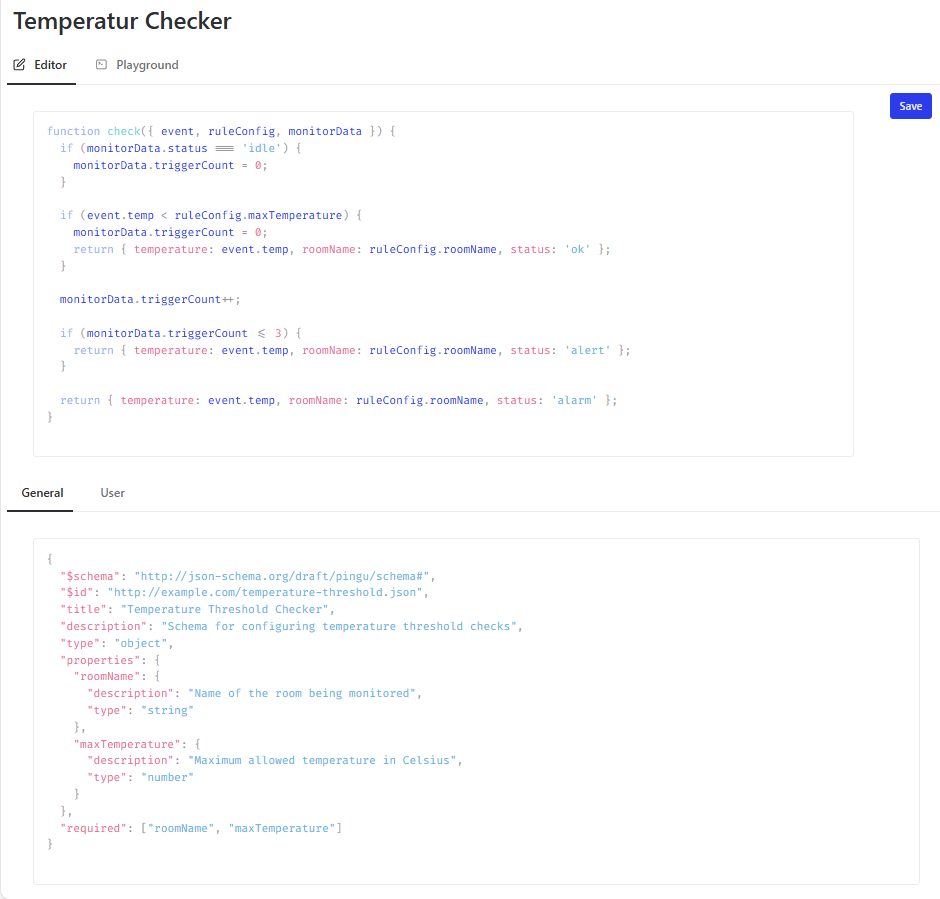
\includegraphics[width=1\linewidth]{function.png}
  \caption{Konfigurationskomponente einer Temperatur Checker Funktion}
  \label{fig:function}
\end{figure}

Nachdem sämtliche Konfigurationskomponenten definiert wurden, erfolgt ihre Zusammenführung in einem Monitor. Abbildung \ref{fig:monitor} zeigt die Eingabemaske zur Erstellung eines Monitors.

In dieser Eingabemaske lassen sich der aktuelle Status (Idle oder Alert), der Aktivitätszustand (Active oder Inactive), eine zuvor definierte Function (z.B. der Temperaturchecker), die gewünschten Actions sowie ein Status-Message-Template auswählen. Der Status gibt den initialen Zustand des Sensors an, der sich während des Betriebs ändern kann. Der Aktivitätszustand legt fest, ob der Sensor aktiv überwacht wird oder inaktiv bleibt. Das Status-Message-Template definiert die Nachricht, die bei einem Alarmstatus von der Monidas-Plattform verwendet wird. Im Bereich Rule Config der Eingabemaske befindet sich ein JSON-Editor, über den die im General-Schema der Function definierten Konfigurationsparameter gesetzt werden können. Diese umfasst ein Textfeld ohne Editorunterstützung. Diese Ansicht ist ab einer Berechtigungsstufe von Systemintegratoren vorgesehen. Alternativ können die User-Konfigurationsparameter nach der Erstellung des Monitors über eine separate Eingabemaske eingegeben werden, welche das User-Schema verwendet und speziell für Endnutzer vorgesehen ist.

\begin{figure}[H]
  \centering
  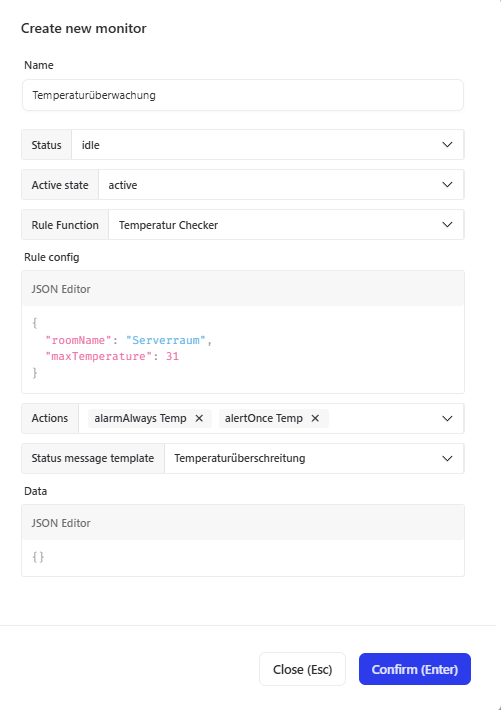
\includegraphics[width=0.7\linewidth]{monitor.png}
  \caption{Eingabemaske zur Erstellung eines Monitors}
  \label{fig:monitor}
\end{figure}

\iffalse
\begin{figure}[H]
  \centering
  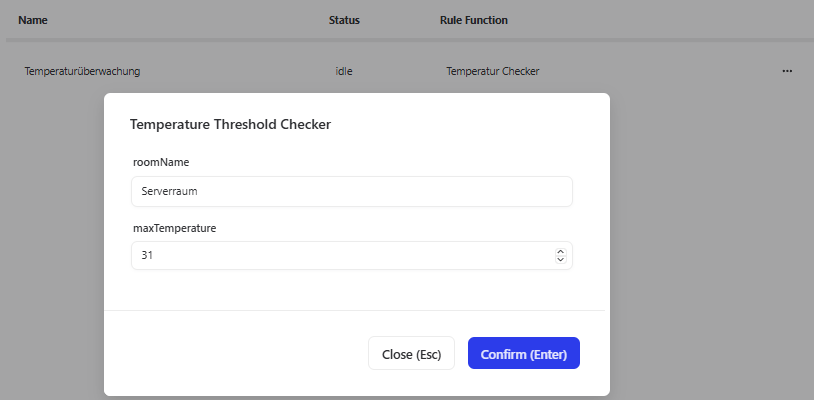
\includegraphics[width=0.7\linewidth]{monitor1.png}
  \caption{Benutzerfreundliche Eingabemaske für Endnutzer}
  \label{fig:monitor1}
\end{figure}
\fi


Nachdem der Monitor vollständig konfiguriert wurde, empfängt und überwacht die Monidas-Plattform kontinuierlich die vom Sensor übermittelten Messwerte. 

Ein Beispiel: Ein Sensor meldet über die API der Plattform einen Temperaturwert von 30 °C. Diese eingehenden Daten werden von der zugeordneten Funktion verarbeitet. Die Funktion prüft, ob der gemeldete Temperaturwert innerhalb des zuvor definierten Grenzwerts liegt. Das Ergebnis dieser Auswertung wird dann im Monitor gespeichert. Dort lässt sich jederzeit ablesen, welchen Zustand (z.B. Status „ok“), welche Temperatur, welcher Raum und weitere Informationen die Auswertung ergeben hat. Somit haben Nutzer jederzeit eine Übersicht über den aktuellen Zustand des überwachten Sensors.

Neben dem hier dargestellten Konfigurationsprozess bietet die Monidas-Plattform Möglichkeiten zur Visualisierung und Auswertung der Sensordaten, etwa in Form von Trendanalysen, Diagrammen oder Übersichten aktueller Alarme. Diese Funktionen sind jedoch nicht Gegenstand dieser Arbeit.

\subsection{Problemstellung}
\label{sec:problemstellung}
Der in Kapitel \ref{kap:konf} beschriebene Konfigurationsprozess erfordert derzeit, dass verschiedene Konfigurationskomponenten in einer festgelegten Reihenfolge erstellt werden. Vor der Einrichtung eines Monitors zur Sensorüberwachung müssen zwingend eine Aktion und eine Funktion definiert werden. Die Aktion setzt voraus, dass zuvor eine Empfängergruppe sowie eine Vorlage für den Inhalt der Benachrichtigung angelegt wurden. Dies hat zur Folge, dass der Systemintegrator mehrere Eingabemasken ausfüllen und miteinander verknüpfen muss, bevor ein Sensor überwacht werden kann.

Je mehr Konfigurationsmöglichkeiten bestehen und je mehr Sensoren überwacht werden, desto höher ist der manuelle Aufwand für den Systemintegrator. Dies wirkt sich langfristig negativ auf die Wartbarkeit und Skalierbarkeit der Plattform aus.


Neben diesem Aufwand gibt es ein weiteres Problem bei der Konfiguration von Function und Monitor. Für diese Konfigurationskomponenten wird ein einfacher Editor verwendet, der keine unterstützenden Funktionen wie Validierung oder Autovervollständigung bietet. Um solche Funktionen direkt in die Monidas-Plattform zu integrieren, müsste die gesamte Editorlogik eigenständig implementiert und gepflegt werden. Dies verursacht erheblichen Entwicklungs- und Wartungsaufwand. Bei externen Entwicklungsumgebungen wie Visual Studio Code hingegen existieren bereits fertige, modulare Erweiterungen. Diese können ohne grossen Aufwand eingebunden und bei Bedarf flexibel angepasst oder erweitert werden.

Zur Reduktion dieses Aufwands wurde im Vorprojekt IP5 („Entwicklung einer VS-Code Extension zur Verwaltung von IoT-Daten \br{wieso jetzt Iot Daten? Kanst du nicht einen Begriff verwende, den du bis jetzt öfters verwendet hast z.b Monitorkonfiugration?}in der Monidas-Plattform“) bereits ein Proof-of-Concept entwickelt, der eine alternative Benutzeroberfläche innerhalb von Visual Studio Code evaluiert. Diese Benutzeroberfläche stellt das Monidas-Datenmodell übersichtlich in einer hierarchischen Baumstruktur (TreeView) dar und ermöglicht eine direkte Bearbeitung der IoT-Daten mittels eines JSON-Editors. Trotz der positiven Ergebnisse des Prototyps offenbarte sich jedoch eine wesentliche Einschränkung: Die Lösung basierte auf einer statischen Integration („Hardcodierung“) des Datenmodells. Dies bedeutete, dass jede Änderung oder Erweiterung manuelle Anpassungen am Quellcode erforderte. Diese starre Implementierung schränkt Flexibilität, Wartbarkeit und Skalierbarkeit deutlich ein und erhöht langfristig den Entwicklungsaufwand.

In dieser Bachelorarbeit wird versucht, die Nachteile der starren Implementierung durch eine generische, datenbankschema-gesteuerte Lösung zu beheben. Dabei beschreibt das Datenbankschema, welche Datentypen gespeichert werden, welche Felder diese enthalten und wie sie miteinander in Beziehung stehen. Neue Funktionen oder Konfigurationskomponenten müssen dadurch nicht mehr einzeln auf der Webplattform implementiert werden, sondern können ausschliesslich durch Anpassungen am Datenmodell bereitgestellt werden. Damit werden die Erweiterbarkeit und Wartbarkeit der Monidas-Plattform deutlich verbessert und der Entwicklungsaufwand signifikant reduziert.

\newpage
\subsection{Monidas Code Assist Navigator}
Der Monidas Code Assist Navigator bietet eine alternative Schnittstelle zur Verwaltung und Konfiguration von Daten innerhalb der Entwicklungsumgebung Visual Studio Code. Die Benutzeroberfläche in VS Code besteht aus zwei Hauptkomponenten: einem Explorer und einem Editor.

Abbildung \ref{fig:res} zeigt, wie der Explorer die Daten übersichtlich in einer Baumstruktur darstellt, während der Editor die Bearbeitung der ausgewählten Daten ermöglicht. Die Ansicht des Explorers basiert auf dem definierten Datenbankschema. Der Editor unterstützt den Benutzer durch den eigens entwickelten Language Server, welcher das Benutzererlebnis durch Funktionen wie Validierung, Autovervollständigung und Navigation innerhalb der Datenbankinstanzen verbessert.


\begin{figure}[H]
  \centering
  \includegraphics[width=\linewidth]{}
  \caption{}
  \label{fig:res}
\end{figure}

\newpage

\subsection{Forschungsfragen}

Die vorliegende Arbeit soll folgende Forschungsfragen beantworten:

\begin{itemize}
    \item Welche Architekturentscheidungen sind erforderlich, um den „Code Assist Navigator“ umzusetzen? 
    \item Welche Auswirkungen hat die Umsetzung des „Code Assist Navigators“ auf die Skalierbarkeit, Erweiterbarkeit und Flexibilität der bestehenden Monidas-Plattform, insbesondere im Hinblick auf das zugrundeliegende Datenbankschema? 
    \item Wo liegen die technischen sowie konzeptionellen Grenzen des „Code Assist Navigators“ bei der Verarbeitung, Darstellung und Navigation komplexer und tiefer Datenmodelle?
\end{itemize}

\subsection{Abgrenzung}
%Im Rahmen dieser Arbeit werden folgende Themenbereiche nicht behandelt. Die entwickelte Lösung wird nicht in das Produktivsystem von Monidas integriert. Es findet keine Anbindung an die bestehende Webplattform oder das Backend statt. Die Evaluation erfolgt ausschliesslich anhand des Datenmodells, ohne produktive Abläufe zu beeinflussen.

% Nicht berücksichtigt werden ausserdem Funktionen zur gleichzeitigen Nutzung durch mehrere Benutzer, die Benutzerverwaltung, Authentifizierungsprozesse sowie die Rechtevergabe. Auch Themen wie Datensicherheit, Performanceoptimierung, Datenmigration oder die Anbindung externer Systeme sind nicht Bestandteil dieser Arbeit.

Im Rahmen dieser Arbeit werden einige Themenbereiche bewusst ausgeklammert. Die entwickelte Lösung wird nicht in das Produktivsystem von Monidas integriert und es erfolgt keine Anbindung an die bestehende Plattform. Die Evaluation der Lösung basiert ausschliesslich auf dem Datenmodell.

Funktionen zur Mehrbenutzernutzung,  Benutzerverwaltung sowie zu Authentifizierungs- und Autorisierungsprozessen bleiben dabei unberücksichtigt. Auch Themen wie Datensicherheit, Performanceoptimierung oder Datenmigration werden im Rahmen dieser Bachelorarbeit nicht weiter behandelt.

\subsection{Leserführung}
In den folgenden Kapiteln werden die einzelnen Aspekte dieses Projekts genauer behandelt.
 
Kapitel \ref{mon} beschäftigt sich mit der Monidas-Plattform. Dabei wird erläutert, wie die Plattform aufgebaut ist, wie das Domänenmodell definiert wurde und welche Technologien eingesetzt wurden. Berücksichtigt werden Technologien, die für die entwickelte Lösung relevant sind.

Kapitel \ref{kap:dbschema} behandelt die Anpassungen am Datenbankschema. Es wird gezeigt, welche zusätzlichen Schema-Anpassungen notwendig sind, um die entwickelte Lösung umzusetzen. Da das ursprüngliche Domänenmodell der Monidas-Plattform sehr umfangreich ist, wird in diesem Kapitel zudem ein vereinfachtes Domänenmodell eingeführt, welches die entwickelte Lösung verständlich und übersichtlich darstellt. Dieses vereinfachte Modell dient als Grundlage für die Erläuterungen in den Kapiteln \ref{kap:vfs} und \ref{kap:lsp}.

Kapitel \ref{kap:vfs}  behandelt das virtuelle Filesystem. Hier wird erläutert, wie das vereinfachte Domänenmodell aus Kapitel \ref{kap:dbschema} genutzt wird, um Daten übersichtlich darzustellen und zu bearbeiten.

Kapitel \ref{kap:lsp} befasst sich mit der Editorunterstützung. Es wird gezeigt, wie durch Integration eines Language Server Protocols Validierung, Autovervollständigung und Navigation innerhalb des Editors umgesetzt werden.

Kapitel \ref{kap:eva} fasst abschliessend die Ergebnisse der vorliegenden Arbeit zusammen. Dabei werden die eingangs formulierten Forschungsfragen beantwortet, die entwickelte Lösung kritisch beurteilt sowie mögliche Erweiterungen aufgezeigt.




